\documentclass[border=10pt]{standalone}
\usepackage{tikz}
\usetikzlibrary{arrows.meta}

\definecolor{sigcolor}{RGB}{0, 120, 200}
\definecolor{dutycolor}{RGB}{0, 120, 200}
\definecolor{gridcolor}{RGB}{200, 200, 200}

\begin{document}
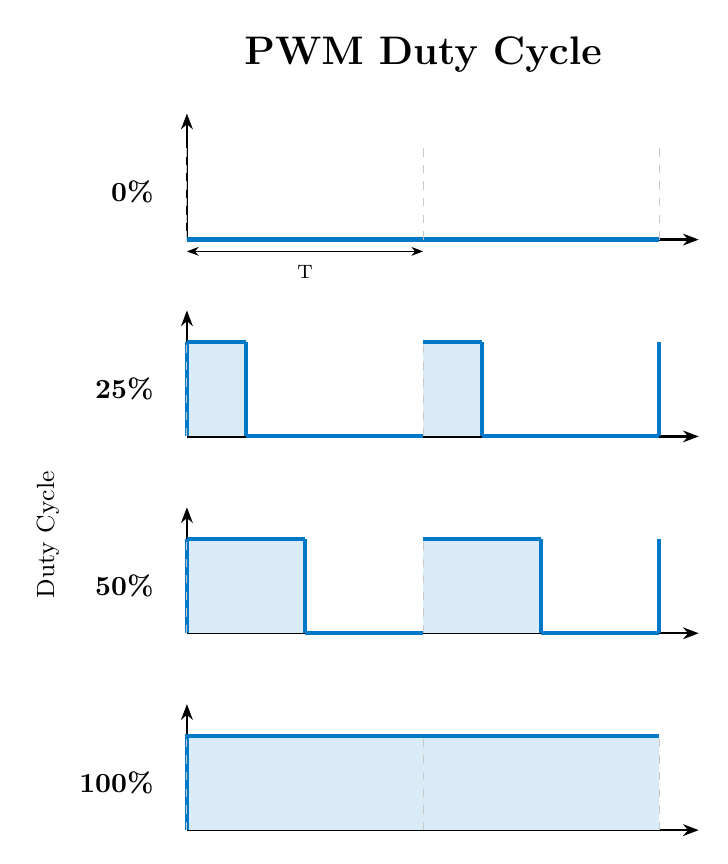
\begin{tikzpicture}[
    axis/.style={-{Stealth[length=2mm]}, line width=0.8pt},
    signal/.style={sigcolor, line width=1.5pt},
    fill area/.style={fill=dutycolor!15},
  ]

  \def\period{3}    % Period width in cm
  \def\height{1.2}  % Signal height in cm
  \def\yspacing{2.5} % Vertical spacing

  % --- 0% Duty ---
  \begin{scope}[yshift=3*\yspacing cm]
    \node[anchor=east, font=\bfseries] at (-0.3, \height/2) {0\%};
    \draw[axis] (0, 0) -- (2*\period+0.5, 0);
    \draw[axis] (0, 0) -- (0, \height+0.4);
    % Signal: always low
    \draw[signal] (0, 0) -- (2*\period, 0);
    % Period markers
    \foreach \i in {0, 1} {
      \draw[gridcolor, dashed] (\i*\period, 0) -- (\i*\period, \height);
    }
    \draw[gridcolor, dashed] (2*\period, 0) -- (2*\period, \height);
    \node[font=\scriptsize, below] at (\period/2, -0.2) {T};
    \draw[{Stealth[length=1.5mm]}-{Stealth[length=1.5mm]}, thin] (0, -0.15) -- (\period, -0.15);
  \end{scope}

  % --- 25% Duty ---
  \begin{scope}[yshift=2*\yspacing cm]
    \node[anchor=east, font=\bfseries] at (-0.3, \height/2) {25\%};
    \draw[axis] (0, 0) -- (2*\period+0.5, 0);
    \draw[axis] (0, 0) -- (0, \height+0.4);
    \foreach \i in {0, 1} {
      \pgfmathsetmacro{\xstart}{\i*\period}
      \pgfmathsetmacro{\xhigh}{\i*\period + 0.25*\period}
      \pgfmathsetmacro{\xend}{(\i+1)*\period}
      % Fill high portion
      \fill[fill area] (\xstart, 0) rectangle (\xhigh, \height);
      % Signal
      \draw[signal] (\xstart, \height) -- (\xhigh, \height)
                     (\xhigh, \height) -- (\xhigh, 0)
                     (\xhigh, 0) -- (\xend, 0);
      \ifnum\i=0
        \draw[signal] (\xstart, 0) -- (\xstart, \height);
      \fi
      % Grid
      \draw[gridcolor, dashed] (\xstart, 0) -- (\xstart, \height);
    }
    \draw[gridcolor, dashed] (2*\period, 0) -- (2*\period, \height);
    \draw[signal] (2*\period, 0) -- (2*\period, \height);
  \end{scope}

  % --- 50% Duty ---
  \begin{scope}[yshift=1*\yspacing cm]
    \node[anchor=east, font=\bfseries] at (-0.3, \height/2) {50\%};
    \draw[axis] (0, 0) -- (2*\period+0.5, 0);
    \draw[axis] (0, 0) -- (0, \height+0.4);
    \foreach \i in {0, 1} {
      \pgfmathsetmacro{\xstart}{\i*\period}
      \pgfmathsetmacro{\xhigh}{\i*\period + 0.5*\period}
      \pgfmathsetmacro{\xend}{(\i+1)*\period}
      \fill[fill area] (\xstart, 0) rectangle (\xhigh, \height);
      \draw[signal] (\xstart, \height) -- (\xhigh, \height)
                     (\xhigh, \height) -- (\xhigh, 0)
                     (\xhigh, 0) -- (\xend, 0);
      \ifnum\i=0
        \draw[signal] (\xstart, 0) -- (\xstart, \height);
      \fi
      \draw[gridcolor, dashed] (\xstart, 0) -- (\xstart, \height);
    }
    \draw[gridcolor, dashed] (2*\period, 0) -- (2*\period, \height);
    \draw[signal] (2*\period, 0) -- (2*\period, \height);
  \end{scope}

  % --- 100% Duty ---
  \begin{scope}[yshift=0cm]
    \node[anchor=east, font=\bfseries] at (-0.3, \height/2) {100\%};
    \draw[axis] (0, 0) -- (2*\period+0.5, 0);
    \draw[axis] (0, 0) -- (0, \height+0.4);
    % Fill entire area
    \fill[fill area] (0, 0) rectangle (2*\period, \height);
    % Signal: always high
    \draw[signal] (0, 0) -- (0, \height) -- (2*\period, \height);
    \foreach \i in {0, 1} {
      \draw[gridcolor, dashed] (\i*\period, 0) -- (\i*\period, \height);
    }
    \draw[gridcolor, dashed] (2*\period, 0) -- (2*\period, \height);
  \end{scope}

  % Title
  \node[font=\Large\bfseries, anchor=south] at (\period, 3*\yspacing + \height + 0.8)
    {PWM Duty Cycle};

  % Axis labels
  \node[font=\small, rotate=90, anchor=south] at (-1.5, 1.5*\yspacing)
    {Duty Cycle};

\end{tikzpicture}
\end{document}
